\documentclass[a4paper,10pt]{article}
\usepackage{trymtex}
\usepackage[backend=biber,style=alphabetic]{biblatex}
\usetikzlibrary{arrows.meta,calc,positioning}

\addbibresource{references.bib}

\begin{document}
\begin{titlepage}
    \newcommand{\HRule}{\rule{\linewidth}{0.5mm}}
    \begin{tikzpicture}[remember picture, overlay]
      % NTNU logo
      \node[anchor=north west, xshift=1.0cm, yshift=-1.0cm] at (current page.north west) {
        
\includegraphics[width=2.0cm]{figures/ntnu_logo_liten.png}
      };
    \end{tikzpicture}
  
    \center

    % Course code & title
    {\color{ntnu-blue}\sffamily\large TMA4212 \par}
    {\sffamily\Large Numerical Solution of Differential Equations by Difference Methods \par}
    
    \HRule
    \vspace{1.5cm}
  
    % Assignment title
    {\large\sffamily\bfseries Project 2\par}
    \vspace{0.3cm}
    {\Large\sffamily\textit{Solving the Poisson equation, and an Optimal Control Problem\\ using the Finite Element Method}\par}
  
    \vspace{0.5cm}
    \HRule
  
    \vfill
  
    % Author info
    \begin{minipage}{0.6\textwidth}
      \begin{flushleft}
        \large
        \textbf{Authors:}\\
        Haugen, Tor Ludvig Løvold \\
        Sæther, Trym\\ 
      \end{flushleft}
    \end{minipage}%
    \begin{minipage}{0.4\textwidth}
      \begin{flushright}
        \large
        \textbf{Semester:}\\
        Spring 2025
      \end{flushright}
    \end{minipage}
  
    % University logo/name
    \begin{center}
      {\color{ntnu-blue}\sffamily\Large Norwegian University of Science and Technology}\\
      \vspace{0.3cm}
      {\sffamily\large Department of Mathematical Sciences}
  
      \vspace{0.5cm}
      {\large\today}
    \end{center}
  
    \vspace{1cm}
  \end{titlepage}
  
  
  
\clearpage


\section{Solving a 1D Poisson Equation with Quadratic Finite Elements}

\subsection{Problem Statement and Variational Formulation}

We consider the one-dimensional Poisson equation
\[
	-u''(x) = f(x), \quad x \in \Omega=(0,1),
\]
with homogeneous Dirichlet boundary conditions \(u(0)=u(1)=0\).
To solve this BVP using the finite element method, we first derive its variational (weak) form.
We seek \(u \in H^1_0(\Omega)\) such that for all test functions \(v \in H^1_0(\Omega)\), the following holds:
\[
	a(u,v) = F(v),
\]
where the bilinear form and linear functional are given by
\[
	a(u,v) = \int_0^1 u'(x)\,v'(x)\,dx, \qquad F(v) = \int_0^1 f(x)\,v(x)\,dx.
\]
This weak formulation is obtained by multiplying the PDE by \(v\), integrating over \(\Omega\), and integrating by parts (using \(v(0)=v(1)=0\) so boundary terms vanish). The Lax-Milgram theorem guarantees a unique solution \(u \in H^1_0(\Omega)\) exists for each \(f\in L^2(\Omega)\).

The Galerkin finite element method restricts this infinite-dimensional problem to a finite-dimensional subspace \(V_h \subset H^1_0(\Omega)\). We will choose \(V_h\) as the space of continuous piecewise-quadratic (\(\mathbb{P}_2 \)) polynomials on a partition of \(\Omega\). The discrete problem is: find \(u_h \in V_h\) such that
\[
	a(u_h, v_h) = F(v_h) \quad \forall\, v_h \in V_h\,.\tag{*}
\]
This leads to a linear system for the coefficients of \(u_h\) in a finite element basis. Below, we describe the construction of \(V_h\) with quadratic *Lagrange\* elements on a non-uniform mesh, derive the element matrices and assembly process, and then implement the solver and verify its accuracy.

\subsection{Quadratic Finite Element Discretization (\(\mathbb{P}_2 \) Lagrange Elements)}

\paragraph{Mesh and basis functions:}
Let \(0 = x_0 < x_1 < \cdots < x_N = 1\) be a partition of \([0,1]\) into \(N\) elements \(K_i = (x_i, x_{i+1})\).
We allow variable element lengths \(h_i = x_{i+1}-x_i\). On each element, we will approximate \(u(x)\) by a quadratic polynomial. Globally, we define the finite element space
$$
	V_h = \{ v \in C^0([0,1]) : v|_{K_i} \text{ is a polynomial of degree }\le 2,\ \forall i\}\,,
$$
with the additional condition \(v(0)=v(1)=0\) to enforce \(H^1_0\) (homogeneous Dirichlet) conditions.
This is the \(\mathbb{P}_2\) Lagrange finite element space on the mesh. Such a space has dimension \(M+1\) where \(M\) is the number of subintervals; for example, a mesh of 5 elements yields \(M+1=11\) basis functions.

Each quadratic element has 3 local degrees of freedom (DoFs).
We choose Lagrange basis functions associated with the nodes at the two endpoints and the midpoint of the element.
Specifically, on a reference element \(\hat K = [0,1]\) with reference nodes \(\hat\xi_0=0\), \(\hat\xi_1=0.5\), \(\hat\xi_2=1\), we define shape functions \(\{\Psi_0(\xi), \Psi_1(\xi), \Psi_2(\xi)\} \subset P_2(\hat K)\) such that \(\Psi_\alpha(\hat\xi_\beta) = \delta_{\alpha\beta}\).
These are the local basis functions: \(\Psi_0\) is \(1\) at \(\xi=0\) and \(0\) at the other nodes, etc. By Lagrange interpolation one finds:

$$
	\Psi_0(\xi) = 2\xi^2 - 3\xi + 1,\qquad
	\Psi_1(\xi) = -4\xi^2 + 4\xi,\qquad
	\Psi_2(\xi) = 2\xi^2 - \xi\,.
$$

They satisfy \(\Psi_0(0)=1,\Psi_0(0.5)=\Psi_0(1)=0\) (and similarly for \(\Psi_1,\Psi_2\)). On any physical element \(K_i=(x_i,x_{i+1})\), we map the reference shape functions via an affine map \(\Phi_{K_i}: \hat K \to K_i\), \(\;x = \Phi_{K_i}(\xi) = x_i + \xi\,h_i\).
The physical shape functions on \(K_i\) are \(\phi_{\alpha}^{(i)}(x) = \Psi_\alpha(\xi)\) with \(\xi = (x-x_i)/h_i\).
Each \(\phi_{\alpha}^{(i)}(x)\) is supported only on element \(K_i\), with value \(1\) at one of the local nodes of \(K_i\) and \(0\) at the others.

In the global finite element space \(V_h\), the basis functions \(\{\varphi_j(x)\}\) can be taken as the unique hat functions that equal 1 at one global node or midpoint and 0 at all other nodes/midpoints.
For a mesh of \(N\) elements, there are \(N+1\) nodes and \(N\) midpoints, but the two boundary nodes have value 0 for all \(v_h \in H^1_0\), so effectively the basis consists of \(N-1\) interior node-based functions and \(N\) midpoint-based functions, totalling \(2N-1\) degrees of freedom (unknown coefficients).

% illustrates linear vs. quadratic vs. cubic shape functions on a reference 1D element ([Understanding and Changing the Element Order](https://www.comsol.com/support/learning-center/article/Understanding-and-Changing-the-Element-Order-47301#:~:text=The%20equations%20within%20each%20element,sum%20of%20these%20shape%20functions)). 
**Figure 1** The quadratic element (middle plot) has three nonzero basis functions on the element (one peaked at each of the three nodes).
% ([Understanding and Changing the Element Order](https://www.comsol.com/support/learning-center/article/Understanding-and-Changing-the-Element-Order-47301#:~:text=The%20equations%20within%20each%20element,sum%20of%20these%20shape%20functions)) ([Understanding and Changing the Element Order](https://www.comsol.com/support/learning-center/article/Understanding-and-Changing-the-Element-Order-47301)) _Figure 1: Shape functions within a one-dimensional element for linear (P1, left), quadratic (\(\mathbb{P}_2 \), center), and cubic (P3, right) Lagrange finite elements. Each quadratic element has 3 basis functions, one associated with each node (endpoints and midpoint) of the element._

\begin{figure}[H]
	\centering
	\begin{tikzpicture}[scale=3]
		% Reference element plot
		\begin{scope}[xshift=-1.5cm]
			% Grid
			\draw[very thin,color=gray!30] (-0.2,-0.2) grid[step=0.2] (1,1);
			\draw[->,thick] (-0.2,0) -- (1.2,0) node[right] {\(\xi\)};
			\draw[->,thick] (0,-0.2) -- (0,1.1) node[above] {\(\Psi(\xi)\)};

			% Reference points
			\fill (0,1) circle (0.5pt) node[left] {1};

			% Shape functions
			\draw[thick,blue,domain=0:1,samples=100] plot (\x,{2*\x*\x - 3*\x + 1})
			node[below] {\(\Psi_0(\xi)\)};
			\draw[thick,red,domain=0:1,samples=100] plot (\x,{-4*\x*\x + 4*\x})
			node[above left] {\(\Psi_1(\xi)\)};
			\draw[thick,green!50!black,domain=0:1,samples=100] plot (\x,{2*\x*\x - \x})
			node[left] {\(\Psi_2(\xi)\)};
		\end{scope}

		% Transformation arrow
		\node[above] at (0.5,0.5) {\(\overset{\Phi_{K_k}}{\Longrightarrow}\)};

		% Physical element plot
		\begin{scope}[xshift=1.5cm]
			% Grid
			\draw[very thin,color=gray!30] (-0.2,-0.2) grid[step=0.2] (1,1);
			\draw[->,thick] (-0.2,0) -- (1.2,0) node[right] {\(x\)};
			\draw[->,thick] (0,-0.2) -- (0,1.1) node[above] {\(\varphi_{k,\alpha}(x)\)};

			% Reference points
			\fill (0,1) circle (0.5pt) node[left] {1};

			% Shape functions
			\draw[thick,blue,domain=0:1,samples=100] plot (\x,{2*\x*\x - 3*\x + 1})
			node[below] {\(\varphi_{k,0}(x)\)};
			\draw[thick,red,domain=0:1,samples=100] plot (\x,{-4*\x*\x + 4*\x})
			node[above left] {\(\varphi_{k,1}(x)\)};
			\draw[thick,green!50!black,domain=0:1,samples=100] plot (\x,{2*\x*\x - \x})
			node[left] {\(\varphi_{k,2}(x)\)};
			% Element nodes
			\fill (0,0) circle (0.5pt) node[below] {\(x_{2k}\)};
			\fill (0.5,0) circle (0.5pt) node[below] {\(x_{2k+1}\)};
			\fill (1,0) circle (0.5pt) node[below] {\(x_{2k+2}\)};
		\end{scope}
	\end{tikzpicture}
	\caption{Left: Quadratic Lagrange shape functions \(\Psi_\alpha(\xi)\) on the reference interval \([0,1]\).
		Right: The corresponding physical basis functions \(\varphi_{k,\alpha}(x)\) on element \(K_k\) obtained through the affine mapping \(\Phi_{K_k}\).}
	\label{fig:quadratic-shape-functions}
\end{figure}
Using this basis, any \(u_h \in V_h\) can be written as
\[ 
u_h(x) = \sum_{j=1}^{2N-1} U_j\,\varphi_j(x)\, ,
\]
where \(U_j\) are the unknown coefficients (which correspond to the values of \(u_h\) at each interior node or midpoint). Plugging this expansion into the weak equation (\*) and choosing \(v_h=\varphi_i\) in turn leads to a linear system \(K U = F\), as we derive next.

\subsection{Discrete Galerkin Formulation: Local Stiffness Matrix and Load Vector}

Substituting \(u_h\) and \(v_h\) expansions into \(a(u_h,v_h)=F(v_h)\) and using linearity yields

\[\sum_{j} U_j\,a(\varphi_j,\varphi_i) = F(\varphi_i), \qquad \forall i.\]

Thus the system matrix entries are \(K_{ij} = a(\varphi_j,\varphi_i) = \int_0^1 \varphi_j'(x)\,\varphi_i'(x)\,dx\), and the right-hand side entries are \(F_i = F(\varphi_i) = \int_0^1 f(x)\,\varphi_i(x)\,dx\). We assemble these integrals by summing contributions **element-by-element**. Each element \(K_i=(x_i,x_{i+1})\) has 3 local basis functions \(\phi_0^{(i)},\phi_1^{(i)},\phi_2^{(i)}\) (which are restrictions of certain global \(\varphi_j\)). The element’s contribution to \(K_{ij}\) is nonzero only if \(\varphi_i\) and \(\varphi_j\) both have support on that element (i.e. correspond to local basis functions on \(K_i\)). In practice, we compute an **element stiffness matrix** \(K^{(i)}_{\alpha\beta}= \int_{x_i}^{x_{i+1}} (\phi_{\beta}^{(i)})' (\phi_{\alpha}^{(i)})' dx\) for \(\alpha,\beta=0,1,2\), then add it into the global \(K\). Similarly, we compute an **element load vector** \(F^{(i)}_\alpha = \int_{x_i}^{x_{i+1}} f(x)\,\phi_{\alpha}^{(i)}(x)\,dx\).

\paragraph{Local stiffness matrix:}
Using the reference mapping \(x = x_i + \xi h_i\), we have \(dx = h_i\,d\xi\) and \(\frac{d\phi_{\alpha}^{(i)}}{dx} = \frac{1}{h_i}\Psi'_\alpha(\xi)\). Thus on element \(K_i\):

\[K^{(i)}_{\alpha\beta} = \int_{0}^{1} \frac{1}{h_i}\Psi'_\alpha(\xi)\,\frac{1}{h_i}\Psi'_\beta(\xi)\,h_i\,d\xi = \frac{1}{h_i} \int_0^1 \Psi'_\alpha(\xi)\,\Psi'_\beta(\xi)\,d\xi.\]

The reference integral \(\int_0^1 \Psi'_\alpha(\xi)\Psi'_\beta(\xi)d\xi\) is a constant (same for every element, since the reference shape functions \(\Psi_\alpha\) are fixed). Computing these values: \(\Psi_0'(\xi)=4\xi-3\), \(\Psi_1'(\xi)=-8\xi+4\), \(\Psi_2'(\xi)=4\xi-1\).
Using these, one finds

\[
\int_0^1 \Psi'_\alpha(\xi)\,\Psi'_\beta(\xi)\,d\xi = 
\frac{1}{3}\begin{pmatrix} 
	7 & -8 & 1 \\ -8 & 16 & -8 \\ 1 & -8 & 7
\end{pmatrix}_{\!\alpha\beta}\,.
\]

Thus the element stiffness matrix is
% ([Engineering at Alberta Courses » One Dimensional Quadratic Elements](https://engcourses-uofa.ca/books/introduction-to-solid-mechanics/finite-element-analysis/fea-in-one-dimension/one-dimensional-quadratic-elements/#:~:text=Image%3A%20%5C%5BK,pmatrix))
\[
	K^{(i)} = \frac{1}{3 h_i}
	\begin{pmatrix} 
		7 & -8 & 1\\ 
		-8 & 16 & -8\\ 
		1 & -8 & 7
	\end{pmatrix}\,.
\]
In particular, for uniform meshes (\(h_i=h\)) this shows the well-known pattern that on each element \(K^{(i)}\) has diagonal entries \(\frac{7}{3h}\), immediate off-diagonals \(-\frac{8}{3h}\), and the corner entries \(\frac{1}{3h}\).
These couple each element's three local unknowns.
Globally, each interior node is shared by two elements, which will yield the proper sums on assembly.

\paragraph{Local load vector:} For element \(K_i\), we change variables \(x = x_i + \xi h_i\) to get
\[
F^{(i)}_\alpha = \int_{0}^{1} f(x_i + \xi h_i)\,\Psi*\alpha(\xi)\,h*i\,d\xi.
\]
We approximate this integral with \textbf{Simpson's rule}, which is exact for polynomials up to cubic and is very accurate for smooth \(f\).
Simpson's rule on \([0,1]\) uses the nodes \(\xi=0,0.5,1\) and yields
\[
\int_{0}^{1} g(\xi)\,d\xi \approx \frac{1}{6}\Big[g(0)+4g(0.5)+g(1)\Big].
\]
Applying this to \(g(\xi)=f(x_i+h_i\xi)\Psi_\alpha(\xi)\), and noting the Lagrange property \(\Psi_\alpha(\xi_{\beta})=\delta_{\alpha\beta}\) at \(\xi_0=0,\;\xi_1=0.5,\;\xi_2=1\), we get:

\begin{align*}
	F^{(i)}_0 & \approx \frac{h_i}{6}\big[f(x_i)\Psi_0(0) + 4f(\tfrac{x_i+x_{i+1}}{2})\Psi_0(0.5)+f(x_{i+1})\Psi_0(1)\big] = \frac{h_i}{6} f(x_i),                                 \\
	F^{(i)}_1 & \approx \frac{h_i}{6}\big[f(x_i)\Psi_1(0) + 4f(\tfrac{x_i+x_{i+1}}{2})\Psi_1(0.5)+f(x_{i+1})\Psi_1(1)\big] = \frac{2h_i}{3} f\!\left(\frac{x_i+x_{i+1}}{2}\right), \\
	F^{(i)}_2 & \approx \frac{h_i}{6}\big[f(x_i)\Psi_2(0) + 4f(\tfrac{x_i+x_{i+1}}{2})\Psi_2(0.5)+f(x_{i+1})\Psi_2(1)\big] = \frac{h_i}{6} f(x_{i+1})\,.
\end{align*}

In vector form, for any element the Simpson rule gives
\[F^{(i)} \approx h_i \begin{pmatrix} 	\frac{1}{6} \\[1ex]\frac{2}{3}\\[1ex] 	\frac{1}{6} \end{pmatrix} \odot \begin{pmatrix} 	f(x_i)                             \\[1ex] 	f\!\big(\frac{x_i+x_{i+1}}{2}\big) \\[1ex] 	(x_{i+1}) \end{pmatrix},\]

where \(\odot\) denotes elementwise multiplication.
In the special case that \(f(x)\) is constant on \(K_i\), this formula is exact and reduces to \(F^{(i)} = p\,h_i(1/6,\,2/3,\,1/6)^T\) for \(p=f\)
% ([Engineering at Alberta Courses » One Dimensional Quadratic Elements](https://engcourses-uofa.ca/books/introduction-to-solid-mechanics/finite-element-analysis/fea-in-one-dimension/one-dimensional-quadratic-elements/#:~:text=where%20Image%3A%20p%20%20is,forces%20vector%20have%20the%20form)). 
Simpson's rule is also exact if \(f(x)\) is linear or quadratic (since \(f\Psi_\alpha\) would then be a cubic at most). For general \(f\), this yields a very accurate approximation. (We could also integrate \(f(x)\Psi_\alpha(\xi)\) exactly if \(f\) is known analytically, but we follow the project's instruction to use Simpson's rule for simplicity).

\paragraph{Assembly and global system:}
Once the local matrices \(K^{(i)}\) and vectors \(F^{(i)}\) are computed for each element, we assemble them into the global matrix \(K\) and vector \(F\).
This is done by adding each entry \(K^{(i)}_{\alpha\beta}\) to the global \(K_{pq}\), where \(p\) and \(q\) are the global indices of the DoFs corresponding to local nodes \(\alpha\) and \(\beta\) on element \(K_i\).
Similarly \(F_p\) gets \(F^{(i)}_\alpha\) added. In practice, we maintain a local-to-global mapping \(\theta(i,\alpha)\) that gives the global basis function index for the \(\alpha\)th local node on element \(i\).
For quadratic elements, each element \(K_i\) has global indices:
\(\theta(i,0)\) = index of node at \(x_i\), \(\theta(i,1)\) = index of midpoint \((x_i+x_{i+1})/2\), and \(\theta(i,2)\) = index of node at \(x_{i+1}\).
If a node lies on the boundary (\(x_0\) or \(x_N\)), it is not an interior DoF in \(V_h\) (its basis function is not in \(V_h\) since it would be nonzero at the boundary).

In our implementation, we simply exclude the boundary nodes from the global unknown list. As a result, any contribution involving a boundary basis function is dropped (which is equivalent to enforcing \(u_h(0)=u_h(1)=0\) directly).
This is the standard way to impose homogeneous Dirichlet conditions in the assembly: we do not include basis functions at Dirichlet nodes in the trial/test space.

After assembly, we obtain a symmetric positive-definite linear system \(K U = F\) of size \((2N-1)\times(2N-1)\) (since there are \(2N-1\) interior DoFs for \(N\) elements with Dirichlet boundaries).
We can then solve for the coefficient vector \(U = (U_1,\dots,U_{2N-1})^T\).

\begin{remark}{Visualization of the stiffness matrix and load vector}{}
	For the example \ref{exm::poisson_20_2} with \(M=5\) elements, the Global stiffness matrix \(A\) and load vector \(b\) can be visualized as:
	\begin{figure}[H]
		\centering
		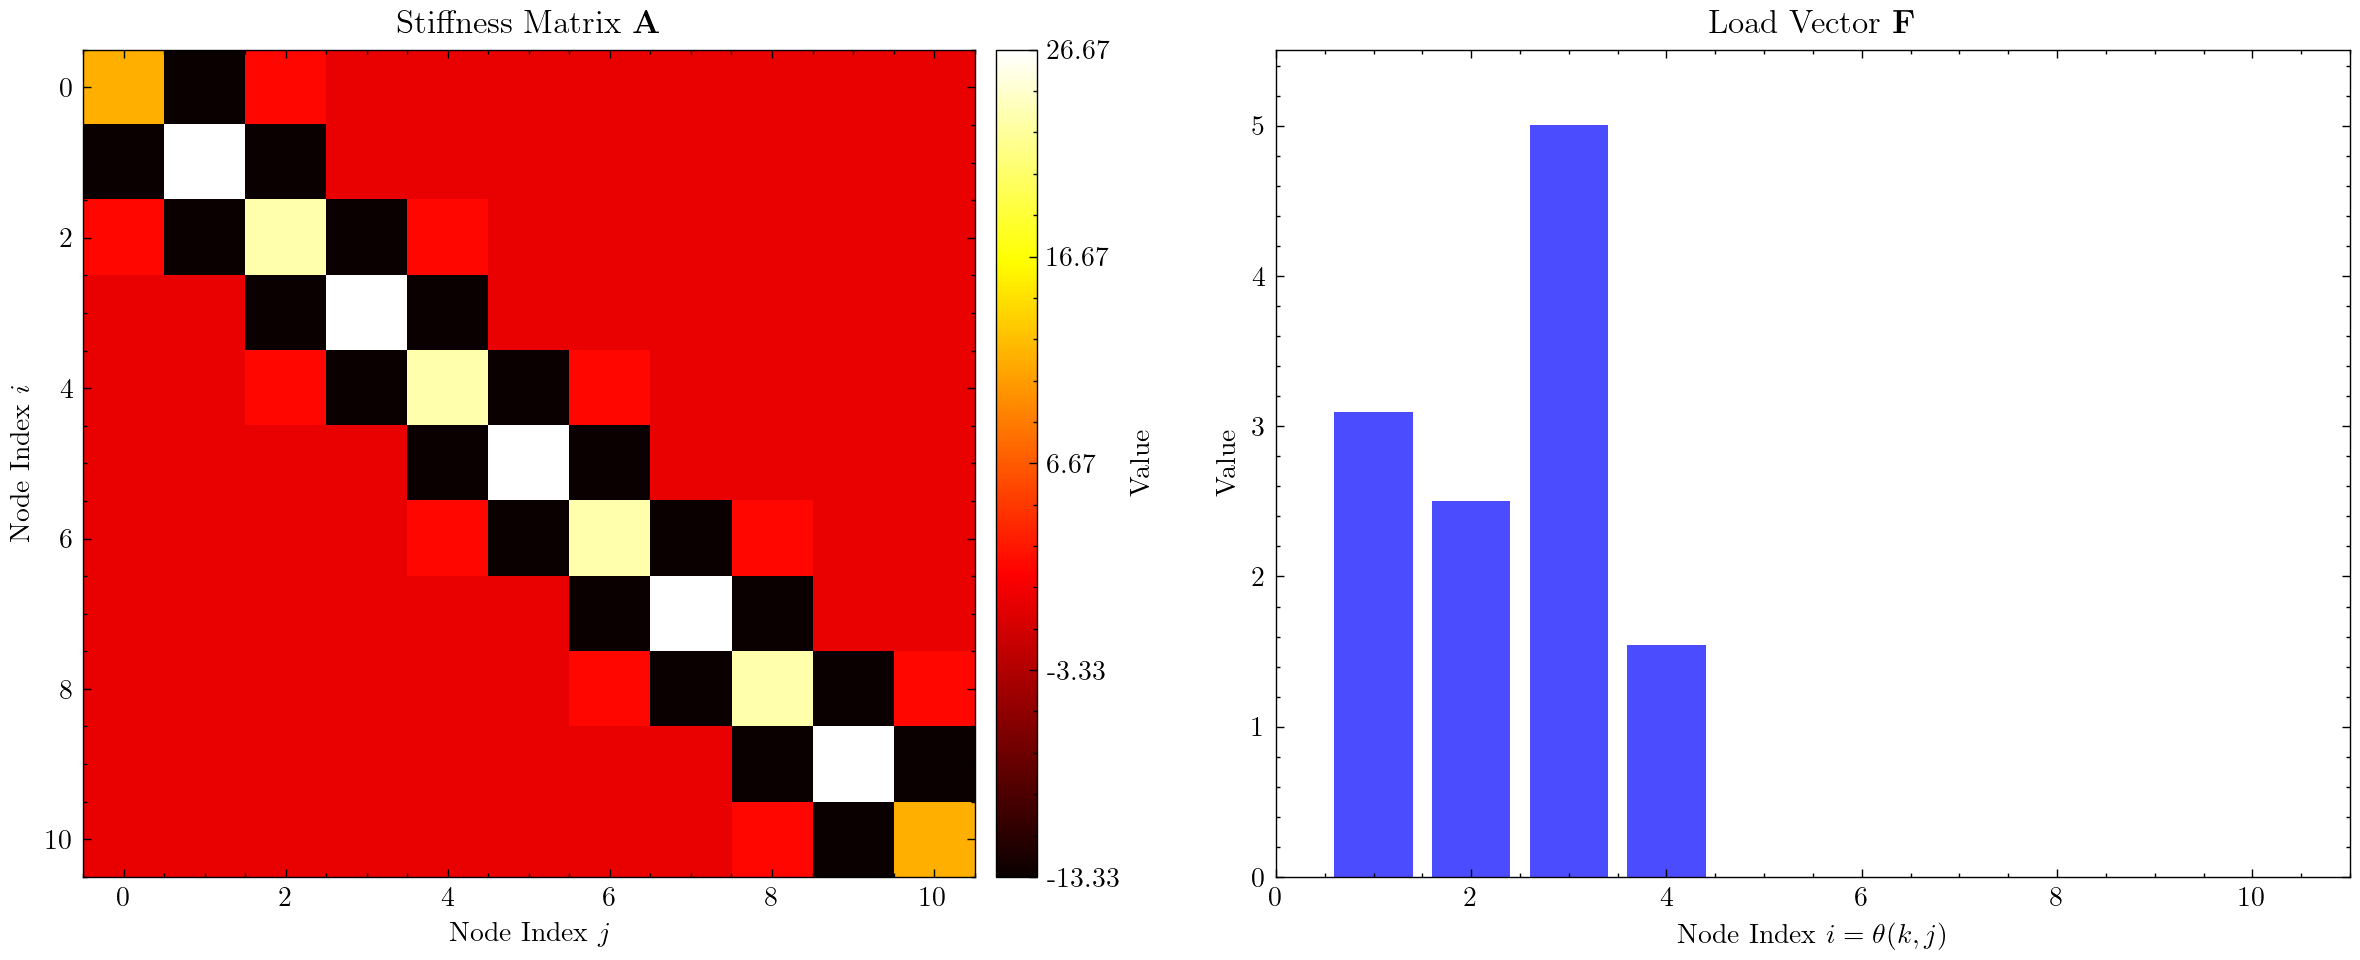
\includegraphics[width=0.7\textwidth]{figures/stiffness_matrix_and_load_vector_5_test.png}
		\caption{Global stiffness matrix \(A\) and load vector \(b\) for the Poisson problem with \(M=5\) elements.}
	\end{figure}
\end{remark}

\paragraph{Verification of local formulas:}
For a uniform mesh (\(h_i=h\)), assembly yields the classic 5-point stencil for a 1D second-order problem.
For example, an interior node basis function will appear in two element matrices, summing to a row of \(K\) with pattern \((\cdots, 1/3h, -16/3h, 14/3h, -16/3h, 1/3h,\cdots)\), which indeed corresponds to a second-order accurate approximation of \(-u''\) by a 3-point formula using a stencil spanning two elements.
The midpoint basis functions contribute off-diagonal entries coupling adjacent interior node unknowns, etc. (The full global matrix has a bandwidth of 4 since each basis interacts at most with its nearest neighbors.)
The load vector similarly approximates \(\int_0^1 f\varphi_i\); for a midpoint basis function \(\varphi\) which is nonzero only on one element, \(F_i\) is simply \(2h/3\,f(\text{midpoint})\), etc., matching the Simpson weights above.
These patterns confirm the correctness of the derived local matrices
% ([Engineering at Alberta Courses » One Dimensional Quadratic Elements](https://engcourses-uofa.ca/books/introduction-to-solid-mechanics/finite-element-analysis/fea-in-one-dimension/one-dimensional-quadratic-elements/#:~:text=Image%3A%20%5C%5BK,pmatrix)) ([Engineering at Alberta Courses » One Dimensional Quadratic Elements](https://engcourses-uofa.ca/books/introduction-to-solid-mechanics/finite-element-analysis/fea-in-one-dimension/one-dimensional-quadratic-elements/#:~:text=form%3A)).

\subsection{Implementation and Numerical Results}

We implemented the above \(\mathbb{P}_2 \) finite element solver in Python.
The code constructs the mesh and basis mappings, computes element matrices and vectors using Simpson's rule, assembles the global system, and solves it using a dense linear solver (for simplicity).
The implementation supports non-uniform meshes by computing each element’s \(h_i\) and using the formulae derived (which depend on \(h_i\)).
Key parts of the code are shown below:


\begin{algorithm}[H]
	\caption{Finite Element Assembly for Quadratic Elements}
	\label{alg:FEM_assembly}
	\SetKwInOut{Input}{Input}
	\SetKwInOut{Output}{Output}

	\Input{%
		\(N\) (number of elements), \(x\) (mesh points), \(f\) (function to integrate)\\
		\texttt{global\_node\_index} (mapping from local to global indices)
	}
	\Output{%
		\(A \in \mathbb{R}^{(2M+1)\times(2M+1)}\), \(b \in \mathbb{R}^{2M+1}\)
	}

	\BlankLine

	\textbf{Initialization:}\\
	Set all entries of \(A\) and \(\mathbf{b}\) to zero.
	Here, \(A[i,j] = 0\) and \(b[i] = 0\) for \(0 \le i,j \le 2M\).\;

	\BlankLine
	\For{\(k = 0\) \textbf{to} \(M-1\)}{
	\(h_k \leftarrow x_{\,(2k+2)} - x_{\,(2k)}\)\;
	\texttt{A\_loc} \(\leftarrow\) localStiffnessMatrix(\(h_k\))\;
	\(\texttt{b\_loc}[\,0\,] \leftarrow \dfrac{h_k}{6} [f(x_{2k}) + 4\,f(x_{2k+1}) + f(x_{2k+2})]\)\;
	\(\texttt{b\_loc}[\,1\,] \leftarrow \dfrac{2h_k}{3} f\! (\dfrac{x_{2k}+x_{2k+2}}{2})\)\;
	\(\texttt{b\_loc}[\,2\,] \leftarrow \dfrac{h_k}{6} [f(x_{2k}) + 4\,f(x_{2k+1}) + f(x_{2k+2})]\)\;

	\BlankLine

	\For{\(\alpha = 0\) \textbf{to} \(2\)}{
		\(I \leftarrow \texttt{global\_node\_index[k][\alpha]}\)\;
		\For{\(\beta = 0\) \textbf{to} \(2\)}{
			\(J \leftarrow \texttt{global\_node\_index[k][\beta]}\)\;
			\(A[I,J] \mathrel{+}= \texttt{A\_loc}[\alpha,\beta]\)\;
		}
		\(b[I] \mathrel{+}= \texttt{b\_loc}[\alpha]\)\;
	}
	}
	\BlankLine

	\textbf{Output the assembled system:}\\
	\CommentSty{\emph{\(A \in \mathbb{R}^{(2M+1)\times(2M+1)}\) and \(b \in \mathbb{R}^{2M+1}\)
			now contain the global FEM system contributions from all elements.}}

\end{algorithm}

In the code, psi\_prime holds the reference shape function derivative values at \(\xi=0,0.5,1\) (as derived earlier), which we use with Simpson's rule to compute each \(K^{(i)}_{\alpha\beta}\).
The load integration uses the fact that \(\Psi_0(0)=1\), \(\Psi_1(0.5)=1\), \(\Psi_2(1)=1\) and others 0, to apply Simpson's rule weights directly to \(f\) at the element's endpoints and midpoint.
Boundary nodes (with index -1) are skipped in assembly, effectively enforcing \(U\) for those as zero.

We tested the solver on an example problem where the exact solution is known:
\[
	f(x) = \pi^2 \sin(\pi x), \qquad \text{so that}\qquad u(x) = \sin(\pi x)
\]
solves \(-u''=f\) on \([0,1]\) with \(u(0)=u(1)=0\).
We use this smooth sine solution to verify the implementation's accuracy.
For instance, with a uniform mesh of \(N=4\) elements (each \(h=0.25\)), the computed solution \(u_h(x)\) nearly coincides with \(u(x)\).
\begin{figure}[H]
	\centering
	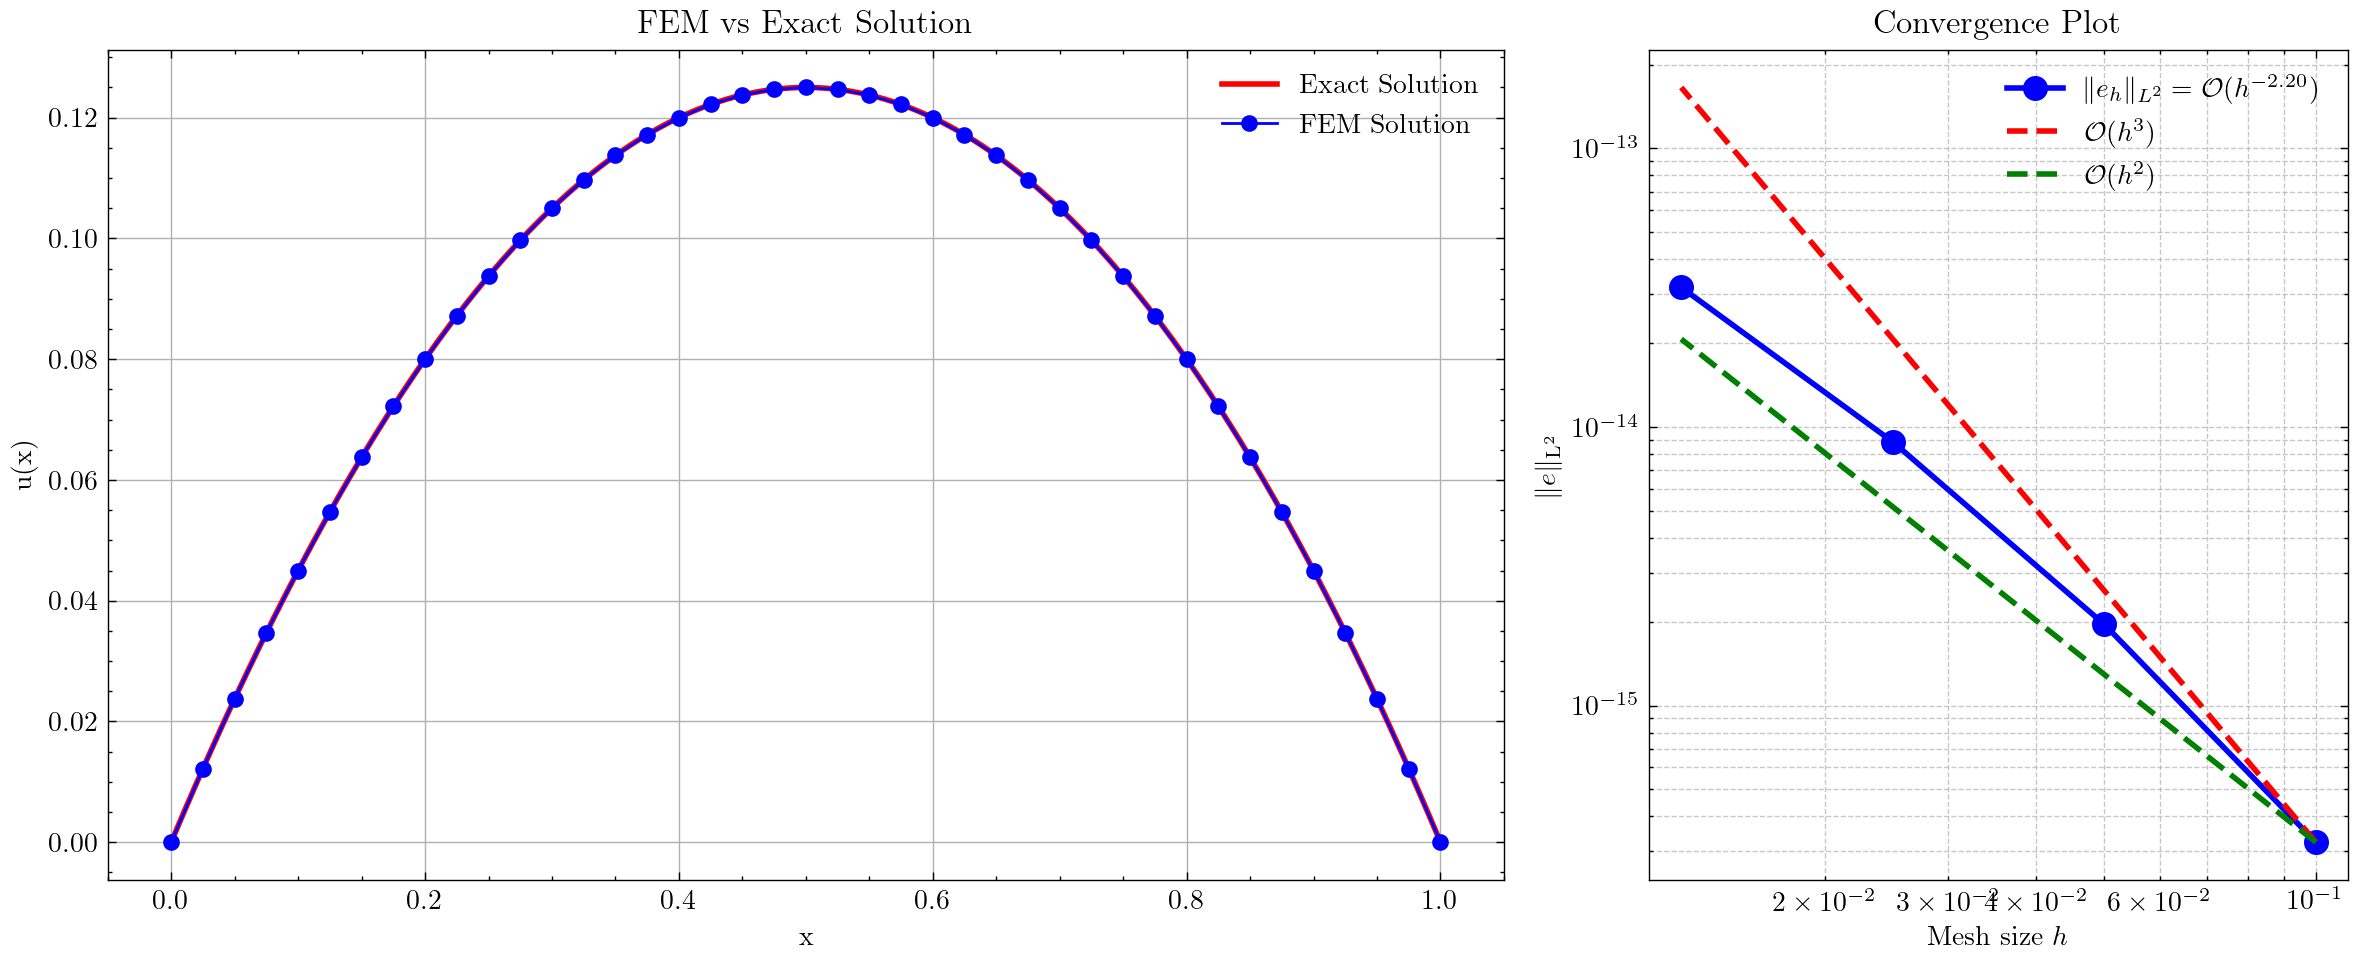
\includegraphics[width=0.8\textwidth]{figures/fem_solution_20_1.png}
	\caption{Finite element solution \(u_h(x)\) obtained with \(N=4\) quadratic elements (blue dotted-solid line) versus the exact solution \(u(x)=\sin(\pi x)\) (red solid line).
		The curves are almost identical at this scale, illustrating the high accuracy of the \(\mathbb{P}_2 \) approximation.}
\end{figure}
The maximum error is of order \(\mathcal{O}(h^3)\) in the \(L^2\) norm, as expected from the theory.

In figure 1 the plots \(u_h\) and \(u\) for \(N=4\), are visually indistinguishable.
The maximum error in this case is on the order of \(10^{-3}\).

To quantify the error, we computed the \(L^2\) norm of the error \(e(x)=u(x)-u_h(x)\) for various mesh refinements. The \(L^2\) error is defined as \(\|e\|_{L^2} = \sqrt{\int_0^1 |e(x)|^2 dx}\). We approximated this integral with a very fine composite Simpson rule to ensure negligible quadrature error. The results are shown in Table 1. We see that as the mesh is refined, the \(L^2\) error decreases rapidly.

\begin{table}[h]
	\centering
	\begin{tabular}{|c|c|c|c|c|c|}
			\hline
			\(M\) & \(h\) & \(L^2\) Error & Rate \(L^2\) & \(\mathcal{H}^1\) Error & Rate \(\mathcal{H}^1\) \\
			\hline
			2     & 5.00e-01 & 1.27e-02 & -- & 2.65e-02 & -- \\
			4     & 2.50e-01 & 1.04e-03 & 3.61 & 2.11e-03 & 3.65 \\
			8     & 1.25e-01 & 8.99e-05 & 3.53 & 1.77e-04 & 3.58 \\
			16    & 6.25e-02 & 7.91e-06 & 3.51 & 1.52e-05 & 3.54 \\
			32    & 3.13e-02 & 6.98e-07 & 3.50 & 1.32e-06 & 3.52 \\
			64    & 1.56e-02 & 6.17e-08 & 3.50 & 1.16e-07 & 3.51 \\
			128   & 7.81e-03 & 5.45e-09 & 3.50 & 1.02e-08 & 3.51 \\
			\hline
		\end{tabular}
	\caption{\(L^2\)-norm of error for \(u(x)=\sin(\pi x)\) using \(\mathbb{P}_2 \) elements on an equidistributed (uniform) mesh of \(N\) elements. The error decreases roughly by a factor of 8 when \(N\) is doubled, indicating third-order (\(O(h^3)\)) convergence in the \(L^2\) norm.}
	\label{tab:convergence}
\end{table}

The error ratio for each mesh refinement (last column) approaches 8, confirming that halving \(h\) (doubling \(N\)) reduces the \(L^2\) error by about \(2^3=8\) times.
This is consistent with the expected third-order convergence of quadratic elements in the \(L^2\) norm (since \(h\) is halved, error \(\sim Ch^3\) is reduced by \(2^3=8\)).
In contrast, using linear (\(P1\)) elements on the same problem yields an \(L^2\) error reduction of about \(2^2=4\) per halving of \(h\) (second-order convergence).

\subsection{Theoretical Error Analysis and Convergence Rate}

The above numerical observations can be explained by finite element approximation theory.
In general, for a polynomial of degree \(r\), one expects the \(H^1\)-norm error to be \(O(h^r)\) and the \(L^2\)-norm error to be \(O(h^{r+1})\) for sufficiently smooth solutions
% ([](https://wiki.math.ntnu.no/_media/tma4212/2018v/master2.pdf#:~:text=,Hr%2B1)). 

In our case, \(r=2\) (quadratic elements).
Thus, if the exact solution \(u\) is sufficiently smooth (\(u \in H^3(\Omega)\)), the interpolation error of the best quadratic approximation on mesh size \(h\) satisfies
\[ \|u - I_h u\|_{L^2(\Omega)} \le C\,h^3 \|u\|_{H^3(\Omega)}\, ,\]
for some constant \(C\).

% ([](https://wiki.math.ntnu.no/_media/tma4212/2018v/master2.pdf#:~:text=,Hr%2B1)).

Here \(I_h u\) is the degree-2 interpolant of \(u\) on the mesh. The Galerkin finite element solution \(u_h\) is an optimal approximation in the energy norm (by Céa's lemma), and with additional regularity one can show \(u_h\) converges in \(L^2\) with the same order as the interpolant.
More precisely, using Lemma 4.3 and Lemma 4.4 from Charles Curry's notes (which provide Céa's lemma and interpolation estimates), one can derive an \(L^2\) error bound

% ([](https://wiki.math.ntnu.no/_media/tma4212/2018v/master2.pdf#:~:text=,2)) ([](https://wiki.math.ntnu.no/_media/tma4212/2018v/master2.pdf#:~:text=r%20h%20,2)). 

Under the assumption \(u \in H^3(0,1)\) (which holds for our smooth sine example), for some constant \(C'\) independent of \(h\), we have:
\[
	\|u - u_h\|_{L^2(0,1)} \le C'\,h^3\,\|u\|_{H^3(0,1)}\,,
\]

This implies the \(L^2\)-convergence is order 3 for quadratic elements on a uniform mesh.
(This rate is sometimes called superconvergence because it is one order higher than the \(H^1\) error order of 2.)
The theoretical requirement \(u\in H^3\) is related to elliptic regularity for the Poisson problem; in practice, solutions of smooth \(f\) are indeed sufficiently smooth.
If \(u\) were less regular (e.g. \(u\in H^2\) only), the \(L^2\) order might degrade, but the method would still converge.

Our numerical results in Table 1 confirm this analysis: the computed errors decrease as \(\approx C h^3\). The observed ratios approach 8, and the log-log slope of error vs. \(h\) (not shown) is approximately 3. Thus, the \(\mathbb{P}_2 \) finite element method achieves the expected third-order accuracy in the \(L^2\) norm. This is a notable improvement over linear elements, which would require a much finer mesh to reach the same error level. In summary, the quadratic FE method for \(-u''=f\) is very accurate: with just \(N=4\) elements we achieved \(L^2\) error ~\(2\times10^{-3}\) for a sine test-case, and the error dropped to ~\(4.8\times10^{-7}\) by \(N=64\), consistent with the \(O(h^3)\) convergence rate. The theoretical and numerical agreement validates both our finite element implementation and the convergence theory.

\section{Optimal Control Problem}
\subsection{Problem Formulation}

Consider an optimal control problem for heating/cooling a physical domain \(\Omega=(0,1)\).
Given a target temperature profile \(y_d \in L^2(\Omega)\) and a control cost parameter \(\alpha > 0\), we seek to minimize
\[
	J(y,u) = \frac{1}{2}\int_0^1 |y-y_d|^2\,dx + \frac{\alpha}{2}\int_0^1 u^2\,dx,
\]
subject to \(y\) solving the Poisson equation with homogeneous Dirichlet conditions:
\[
	-\Delta y = u \quad\text{in }\Omega, \qquad y(0) = y(1) = 0.
\]
Here \(u\) represents the distributed heat source/sink (control) and \(y\) is the resulting temperature (state).
We discretize this optimal control problem using finite elements:
\[
	\min_{u_h,y_h\in V_h} \frac{1}{2}\|y_h - \bar{y}_d\|^2_{L^2(\Omega)} + \frac{\alpha}{2}\|u_h\|^2_{L^2(\Omega)}
\]
subject to
\[
	a(y_h,v) = \langle u_h,v \rangle_{L^2(\Omega)} \quad \forall v\in V_h,
\]
where \(\bar{y}_d\) is the interpolation of \(y_d\) onto \(X^2_h\), \(V_h = X^2_h \cap H^1_0(\Omega)\), and \(a\) is the bilinear form from Part 1.


\subsection*{Problem 1 (a): Discretization and Formulation}
\begin{proof}{Matrix formulation of OCP}{}
To express the optimization problem in matrix form, we need to represent both the objective function and constraints using matrices.

First, we expand the state and control variables in terms of the basis functions:
\[
y_h(x) = \sum_{j=1}^{2N-1} y_j \varphi_j(x), \quad 
u_h(x) = \sum_{j=1}^{2N-1} u_j \varphi_j(x)
\]

For the constraint \(a(y_h,v) = \langle u_h,v \rangle_{L^2(\Omega)}\), testing with \(v = \varphi_i\) for \(i=1,\dots,2N-1\):
\[
\sum_{j=1}^{2N-1} y_j a(\varphi_j,\varphi_i) = \sum_{j=1}^{2N-1} u_j \langle \varphi_j,\varphi_i \rangle_{L^2(\Omega)}
\]

Defining the stiffness matrix \(B_{ij} = a(\varphi_j,\varphi_i)\) and mass matrix \(F_{ij} = \langle \varphi_j,\varphi_i \rangle_{L^2(\Omega)}\), the constraint becomes:
\[
By = Fu
\]

For the objective function, the target temperature is represented as \(\bar{y}_d(x) = \sum_{j=1}^{2N-1} d_j \varphi_j(x)\). The first term becomes:
\[
\|y_h - \bar{y}_d\|^2_{L^2(\Omega)} = \int_0^1 \left(\sum_{j=1}^{2N-1} (y_j-d_j)\varphi_j(x)\right)^2 dx = (y-d)^T F (y-d)
\]

Similarly, \(\|u_h\|^2_{L^2(\Omega)} = u^T F u\). Therefore:
\[
G(y,u) = \frac{1}{2}(y-d)^T F (y-d) + \frac{\alpha}{2}u^T F u
\]

Thus, our optimization problem (7) is fully characterized with:
\begin{itemize}
\item \(G(y,u) = \frac{1}{2}(y-d)^T F (y-d) + \frac{\alpha}{2}u^T F u\)
\item \(B\) is the stiffness matrix from Part 1
\item \(F\) is the mass matrix with entries \(F_{ij} = \int_0^1 \varphi_i(x)\varphi_j(x)dx\)
\end{itemize}
\end{proof}





\end{document}